%!TEX program = xelatex
\documentclass[11pt]{beamer}

\usepackage{amsfonts}
\usepackage{amsmath}
\usepackage{blindtext}
\usepackage{enumitem}
\usepackage{fancyvrb}
\usepackage{tikz}

\usetheme{SaoPaulo}

\title{Numerical Python}
\subtitle{plotting, arrays}
\author{CS101 Lecture \#15}
\date{2016-10-19}

\setcounter{showSlideNumbers}{1}

\newcommand{\correctstar}{\textcolor{red}{$\star$}}

\begin{document}
  \setcounter{showProgressBar}{0}
  \setcounter{showSlideNumbers}{0}

%%%%%%%%%%%%%%%%%%%%%%%%%%%%%%%%%%%%%%%%%%%%%%%%%%%%%%%%%%%%%%%%%%%%%%%%%%%%%%%%
\frame{\titlepage}

%%%%%%%%%%%%%%%%%%%%%%%%%%%%%%%%%%%%%%%%%%%%%%%%%%%%%%%%%%%%%%%%%%%%%%%%%%%%%%%%
\setcounter{framenumber}{0}
\setcounter{showProgressBar}{1}
\setcounter{showSlideNumbers}{1}

%%%%%%%%%%%%%%%%%%%%%%%%%%%%%%%%%%%%%%%%%%%%%%%%%%%%%%%%%%%%%%%%%%%%%%%%%%%%%%%%
\section{Administrivia}

%%%%%%%%%%%%%%%%%%%%%%%%%%%%%%%%%%%%%%%%%%%%%%%%%%%%%%%%%%%%%%%%%%%%%%%%%%%%%%%%
\begin{frame}
  \frametitle{Administrivia}
  \Enlarge

  \begin{itemize}
  \myitem  Homework \#8 is due Monday, Oct.\ 24.
  \myitem  Office hours change from Wed to Thu this week (check website).
  \end{itemize}
\end{frame}

%%%%%%%%%%%%%%%%%%%%%%%%%%%%%%%%%%%%%%%%%%%%%%%%%%%%%%%%%%%%%%%%%%%%%%%%%%%%%%%%
\section{Warmup Quiz}

%%%%%%%%%%%%%%%%%%%%%%%%%%%%%%%%%%%%%%%%%%%%%%%%%%%%%%%%%%%%%%%%%%%%%%%%%%%%%%%%
\begin{frame}[fragile]
  \frametitle{Question \#1}
  \Enlarge

  \begin{Verbatim}
NameError:  name 'y' is not defined.
  \end{Verbatim}

  Which of the following produces this error?

  \begin{enumerate}[label=\Alph*]
  \item
  \begin{Verbatim}
x = 1
y = x * 2
  \end{Verbatim}
  \item
  \begin{Verbatim}
x = 0
y += 1
  \end{Verbatim}
  \item
  \begin{Verbatim}
x = 'ABCD'
y = x[ 2 ]
  \end{Verbatim}
  \end{enumerate}
\end{frame}

%%%%%%%%%%%%%%%%%%%%%%%%%%%%%%%%%%%%%%%%%%%%%%%%%%%%%%%%%%%%%%%%%%%%%%%%%%%%%%%%
\begin{frame}[fragile]
  \frametitle{Question \#1}
  \Enlarge

  \begin{Verbatim}
NameError:  name 'y' is not defined.
  \end{Verbatim}

  Which of the following produces this error?

  \begin{enumerate}[label=\Alph*]
  \item
  \begin{Verbatim}
x = 1
y = x * 2
  \end{Verbatim}
  \item  \correctstar
  \begin{Verbatim}
x = 0
y += 1
  \end{Verbatim}
  \item
  \begin{Verbatim}
x = 'ABCD'
y = x[ 2 ]
  \end{Verbatim}
  \end{enumerate}
\end{frame}

%%%%%%%%%%%%%%%%%%%%%%%%%%%%%%%%%%%%%%%%%%%%%%%%%%%%%%%%%%%%%%%%%%%%%%%%%%%%%%%%
\begin{frame}[fragile]
  \frametitle{Question \#2}
  \Enlarge

  \begin{Verbatim}
IndexError:  list index out of range.
  \end{Verbatim}

  Which of the following produces this error?

  \begin{enumerate}[label=\Alph*]
  \item
  \begin{Verbatim}
x = 'ABCD' + 'E'
x[ 5 ]
  \end{Verbatim}
  \item
  \begin{Verbatim}
x = [ 1,2 ]
x[2]
  \end{Verbatim}
  \item
  \begin{Verbatim}
x = { 1:2, 2:3 }
y = x[2]
  \end{Verbatim}
  \end{enumerate}
\end{frame}

%%%%%%%%%%%%%%%%%%%%%%%%%%%%%%%%%%%%%%%%%%%%%%%%%%%%%%%%%%%%%%%%%%%%%%%%%%%%%%%%
\begin{frame}[fragile]
  \frametitle{Question \#2}
  \Enlarge

  \begin{Verbatim}
IndexError:  list index out of range.
  \end{Verbatim}

  Which of the following produces this error?

  \begin{enumerate}[label=\Alph*]
  \item
  \begin{Verbatim}
x = 'ABCD' + 'E'
x[ 5 ]
  \end{Verbatim}
  \item  \correctstar
  \begin{Verbatim}
x = [ 1,2 ]
x[2]
  \end{Verbatim}
  \item
  \begin{Verbatim}
x = { 1:2, 2:3 }
y = x[2]
  \end{Verbatim}
  \end{enumerate}
\end{frame}

%%%%%%%%%%%%%%%%%%%%%%%%%%%%%%%%%%%%%%%%%%%%%%%%%%%%%%%%%%%%%%%%%%%%%%%%%%%%%%%%
\begin{frame}[fragile]
  \frametitle{Question \#3}
  \Enlarge

  \begin{Verbatim}
SyntaxError:  invalid syntax.
  \end{Verbatim}

  Which of the following produces this error?

  \begin{enumerate}[label=\Alph*]
  \item
  \begin{Verbatim}
if x < 'HAPPY':
  print(x.lower()[1])
  \end{Verbatim}
  \item
  \begin{Verbatim}
if x in 'ABCD':
  print( 'E' + x[ 0 ] )
  \end{Verbatim}
  \item
  \begin{Verbatim}
if x = ( 1,2,3 ):
  print( x[2] + 1 )
  \end{Verbatim}
  \end{enumerate}
\end{frame}

%%%%%%%%%%%%%%%%%%%%%%%%%%%%%%%%%%%%%%%%%%%%%%%%%%%%%%%%%%%%%%%%%%%%%%%%%%%%%%%%
\begin{frame}[fragile]
  \frametitle{Question \#3}
  \Enlarge

  \begin{Verbatim}
SyntaxError:  invalid syntax.
  \end{Verbatim}

  Which of the following produces this error?

  \begin{enumerate}[label=\Alph*]
  \item
  \begin{Verbatim}
if x < 'HAPPY':
  print(x.lower()[1])
  \end{Verbatim}
  \item
  \begin{Verbatim}
if x in 'ABCD':
  print( 'E' + x[ 0 ] )
  \end{Verbatim}
  \item  \correctstar
  \begin{Verbatim}
if x = ( 1,2,3 ):
  print( x[2] + 1 )
  \end{Verbatim}
  \end{enumerate}
\end{frame}

%%%%%%%%%%%%%%%%%%%%%%%%%%%%%%%%%%%%%%%%%%%%%%%%%%%%%%%%%%%%%%%%%%%%%%%%%%%%%%%%
\section{Numerical Python (\texttt{numpy})}

%%%%%%%%%%%%%%%%%%%%%%%%%%%%%%%%%%%%%%%%%%%%%%%%%%%%%%%%%%%%%%%%%%%%%%%%%%%%%%%%
\begin{frame}[fragile]
  \frametitle{The problem}
  \Enlarge

  \begin{Verbatim}
mydata = [ 4.5, 6.0, 1.2, 5.4 ]
from math import sin
sin(mydata)
  \end{Verbatim}
  %\pause
  \begin{enumerate}
  \myitem  Why doesn't this work? %\pause
  \mysubitem  \texttt{list} can contain any type!
  \myitem  Also operators don't do what we ``want":
  \end{enumerate}
  \begin{Verbatim}
mydata * 2.0  # doesn't double values!
  \end{Verbatim}
\end{frame}

%%%%%%%%%%%%%%%%%%%%%%%%%%%%%%%%%%%%%%%%%%%%%%%%%%%%%%%%%%%%%%%%%%%%%%%%%%%%%%%%
\begin{frame}[fragile]
  \frametitle{\texttt{numpy}}
  \Enlarge

  \begin{Verbatim}
import numpy
import numpy as np  # better way
  \end{Verbatim}
  %\pause
  \begin{enumerate}
  \myitem  \texttt{numpy} provides arrays and mathematical functions.
  \end{enumerate}
  \begin{Verbatim}
data = np.array( [ 4.5, 6.0, 1.2, 5.4 ] )
data * 2.0
  \end{Verbatim}
\end{frame}

%%%%%%%%%%%%%%%%%%%%%%%%%%%%%%%%%%%%%%%%%%%%%%%%%%%%%%%%%%%%%%%%%%%%%%%%%%%%%%%%
\begin{frame}[fragile]
  \frametitle{\texttt{numpy}}
  \Enlarge

  Consider a data set containing patient inflammation records for 60 patients over a period of 40 days, contained in \texttt{inflammation.csv}.

  \begin{Verbatim}
  data = np.loadtxt( './data/inflammation.csv',
                     delimiter=',' )
  \end{Verbatim}
\end{frame}

%%%%%%%%%%%%%%%%%%%%%%%%%%%%%%%%%%%%%%%%%%%%%%%%%%%%%%%%%%%%%%%%%%%%%%%%%%%%%%%%
\begin{frame}[fragile]
  \frametitle{\texttt{numpy}}
  \Enlarge

  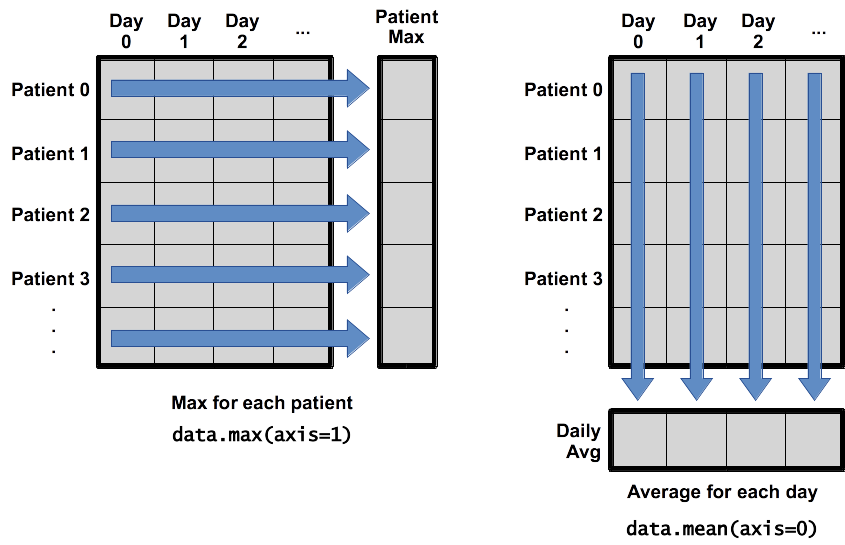
\includegraphics[width=\textwidth]{./img/axes.png}
\end{frame}

%%%%%%%%%%%%%%%%%%%%%%%%%%%%%%%%%%%%%%%%%%%%%%%%%%%%%%%%%%%%%%%%%%%%%%%%%%%%%%%%
\section{Plotting (\texttt{matplotlib})}

%%%%%%%%%%%%%%%%%%%%%%%%%%%%%%%%%%%%%%%%%%%%%%%%%%%%%%%%%%%%%%%%%%%%%%%%%%%%%%%%
\begin{frame}[fragile]
  \frametitle{\texttt{matplotlib}}
  \Enlarge

  \begin{Verbatim}
import matplotlib.pyplot as plt
%matplotlib inline               # jupyter only
  \end{Verbatim}
  %\pause
  \begin{enumerate}
  \myitem  A plotting environment similar to MATLAB.
  \myitem  Can plot \texttt{list}s or \texttt{array}s.
  \end{enumerate}
  \begin{Verbatim}
xs = list( range(4) )
ys = [ 4.5, 6.0, 1.2, 5.4 ]
plt.plot( xs, ys )
plt.show()
  \end{Verbatim}
\end{frame}

%%%%%%%%%%%%%%%%%%%%%%%%%%%%%%%%%%%%%%%%%%%%%%%%%%%%%%%%%%%%%%%%%%%%%%%%%%%%%%%%
\begin{frame}[fragile]
  \frametitle{\texttt{matplotlib}}
  \Enlarge

  \begin{enumerate}
  \myitem  \emph{Always} include labels:
  \mysubitem  \texttt{plt.xlabel( 'domain' )}
  \mysubitem  \texttt{plt.ylabel( 'range' )}
  \mysubitem  \texttt{plt.title( 'topical data' )}
  \end{enumerate}
  \begin{Verbatim}
plt.plot( xs, ys )
plt.xlabel( 'x' )
plt.ylabel( 'y' )
plt.title( 'some values' )
plt.show()
  \end{Verbatim}
\end{frame}

%%%%%%%%%%%%%%%%%%%%%%%%%%%%%%%%%%%%%%%%%%%%%%%%%%%%%%%%%%%%%%%%%%%%%%%%%%%%%%%%
\begin{frame}[fragile]
  \frametitle{\texttt{matplotlib}}
  \Enlarge

  \begin{enumerate}
  \myitem  Basic cycle:
    \begin{enumerate}
    \mysubitem  Add data to plot.
    \mysubitem  Add labels to plot.
    \mysubitem  Show plot.
    \end{enumerate}
  \end{enumerate}
\end{frame}

%%%%%%%%%%%%%%%%%%%%%%%%%%%%%%%%%%%%%%%%%%%%%%%%%%%%%%%%%%%%%%%%%%%%%%%%%%%%%%%%
\begin{frame}[fragile]
  \frametitle{\texttt{matplotlib}}
  \Enlarge

  \begin{enumerate}
    \myitem  Two kinds of plots today:
    \mysubitem  \texttt{plt.plot( x, y )  \# for ptwise data}
    \mysubitem  \texttt{plt.imshow( A )   \# for array data}
    %\pause
    \myitem  \texttt{plot}:  third argument is \emph{format string} (optional).
  \end{enumerate}
  \begin{Verbatim}
plt.plot( xs, ys, 'r.' )
plt.show()
  \end{Verbatim}
  %\pause
  \begin{enumerate}
    \myitem  \texttt{plot}:  can also take keyword arguments.
  \end{enumerate}
  \begin{Verbatim}
plt.plot( xs, ys, 'r.', label='height' )
plt.show()
  \end{Verbatim}
\end{frame}

%%%%%%%%%%%%%%%%%%%%%%%%%%%%%%%%%%%%%%%%%%%%%%%%%%%%%%%%%%%%%%%%%%%%%%%%%%%%%%%%
\section{Reminders}

%%%%%%%%%%%%%%%%%%%%%%%%%%%%%%%%%%%%%%%%%%%%%%%%%%%%%%%%%%%%%%%%%%%%%%%%%%%%%%%%
\begin{frame}
  \frametitle{Reminders}
  \Enlarge

  \begin{itemize}
  \myitem  Homework \#8 is due Monday, Oct.\ 24.
  \myitem  Office hours change from Wed to Thu this week (check website).
  \end{itemize}
\end{frame}

\end{document}
